\chapter{Travail réalisé}
\label{chap:realisation}

Nous commencerons par utiliser la base de données des vins blancs, car celles-ci contiennent le plus grand nombre d'exemples.
Puis nous allons utiliser la base de données des vins rouges qui contient moins d'exemples, afin de vérifier l'impact
du nombre d'exemples sur les performances.

Chaque base de données est séparée en deux parties~: la partie d'entrainement et la partie de test. Les données ont également
été normalisées.


\section{K-nearest neighbors}
\label{sec:knn}

\subsection*{Caractéristiques complètes}
\label{par:dataset-complet-knn}

Le principe des K-nearest neighbors est de classer un objet par rapport aux objets qui sont le plus proche de lui.
Appliqué à la classification de vins, un algorithme KNN observera tous les vins ayant des propriétés similaires. Il
quelle qualité est attribuée à ces vins similaires afin de déterminer la qualité du vin observé.

Lors des tests, nous avons obtenu une précision de 0.62 sur la base d'apprentissage et une précision de 0.55 sur la
base de test en prenant 10 voisins. En diminuant le nombre de voisins à 3, nous obtenons une précision de 0.77 sur la
base d'apprentissage et 0.56 sur la base de test. Au contraire, augmenter le nombre de voisins à 20 diminue la précision
à 0.58 sur la base d'apprentissage et 0.54 sur la base de test.

Nous constatons qu'augmenter le nombre de voisins diminue les performances en apprentissage. En revanche, la précision
en validation ne varie que très peu. L'algorithme KNN reste cependant relativement simple, pour améliorer ces résultats, nous pouvons changer de modèle.

\subsection*{Caractéristiques limitées}
\label{par:dataset-limit-knn}

En limitant le nombre de caractéristiques, on obtient une précision de 0.76 sur la base d'apprentissage et 0.51 sur la base de test avec 3 voisins.
Avec 10 voisins, nous obtenons une précision de 0.61 sur la base d'apprentissage et 0.53 sur la base de test. Et avec 20 voisins, nous obtenons une
précision de 0.59 sur la base d'apprentissage et 0.55 sur la base de test.

Nous constatons que le nombre de voisins a toujours la même influence sur les performances, mais diminuer le nombre de caractéristiques a permis d'améliorer
considérablement les performances en apprentissage et de les améliorer légèrement en validation.

\section{SVM}
\label{sec:svm}

\subsection*{Caractéristiques complètes}
\label{par:dataset-complet-svm}

Le principe des SVM consiste à ramener un problème de classification ou de discrimination à un \textbf{hyperplan} (\textit{feature space})
dans lequel les données sont séparées en plusieurs classes dont la frontière est la plus éloignée possible des points de
données (ou "marge maximale"). D'où l'autre nom attribué aux SVM : les séparateurs à vaste marge. Le concept de frontière
implique que les données soient linéairement séparables. Pour y parvenir, les support vector machines font appel à des noyaux,
c'est-à-dire des fonctions mathématiques permettant de projeter et séparer les données dans l'espace vectoriel, les "vecteurs
de support" étant les données les plus proches de la frontière. C'est la frontière la plus éloignée de tous les points d'entraînement
qui est optimale, et qui présente donc la meilleure capacité de généralisation.

Nous avons obtenu une précision de 0.54 en apprentissage et 0.53 en validation. Les performances obtenues sont légèrement inférieures à
celles l'algorithme KNN, cela est peut-être dû au grand nombre de caractéristiques. Nous retesterons cet algorithme avec un nombre inférieur
de caractéristiques.

\subsection*{Caractéristiques limitées}
\label{par:dataset-limit-svm}

En diminuant le nombre de caractéristiques, nous obtenons une précision de 0.53 sur la base d'apprentissage et 0.53 sur la base de test. Ce résultat
est quasi identique à celui obtenu avec les données complètes, le nombre de caractéristiques n'a donc aucun impact sur les performances des SVM.

\section{Réseau de neurones}
\label{sec:neurones}

\subsection*{Classification}
\label{sec:classification}

Les réseaux de neurones sont une technique d'apprentissage supervisé pouvant répondre à différents problèmes tels que
la classification ou la régression.

Tous les entrainements ont été effectués sur 300 époques avec un modèle composé de 2 couches cachées de 12 neurones chacune.

\subsubsection*{Caractéristiques complètes}
\label{par:dataset-complet-neurones}

Avec en utilisant toutes les caractéristiques, nous obtenons une précision de 0.6 en apprentissage et 0.55 en validation (\textit{Fig.}
\ref{fig:full-class-accuracy-white}) avec une perte de 1.0 en apprentissage et 1.1 en validation (\textit{Fig.} \ref{fig:full-class-loss-white}).
Ces résultats sont assez moyens, mais ne semble pas indiquer un sur-apprentissage.

\begin{figure}[ht]
	\centering
	\begin{minipage}[t]{0.48\textwidth}
		\centering
		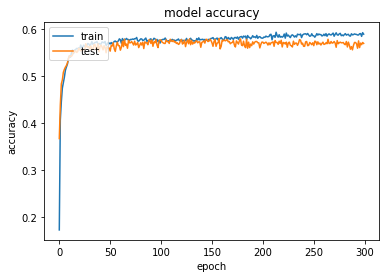
\includegraphics[scale=0.475]{../images/vins_blancs/full_class_accuracy_white.png}
		\caption[Précision du réseau avec toutes les caractéristiques.]
		{\textbf{Précision du réseau avec toutes les caractéristiques}.}
		\label{fig:full-class-accuracy-white}
	\end{minipage}\hfill
	\begin{minipage}[t]{0.48\textwidth}
		\centering
		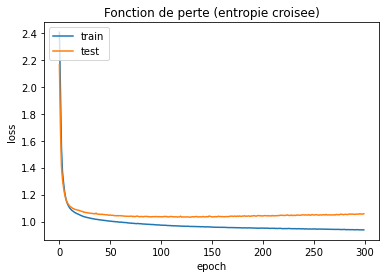
\includegraphics[scale=0.475]{../images/vins_blancs/full_class_loss_white.png}
		\caption[Fonction de perte du réseau avec toutes les caractéristiques.]
		{\textbf{Fonction de perte du réseau avec toutes les caractéristiques}.}
		\label{fig:full-class-loss-white}
	\end{minipage}
\end{figure}

\subsubsection*{Caractéristiques limitées}
\label{par:dataset-limitee-neurones}

En réduisant le nombre de caractéristiques, nous obtenons des performances similaires, nous obtenons une précision de 0.58 en apprentissage
et 0.55 en validation (\textit{Fig.} \ref{fig:small-class-accuracy-white}) avec une perte de 1.0 en apprentissage et 1.1 en validation
(\textit{Fig.} \ref{fig:small-class-loss-white}). Cela montre qu'il y a eu un sous-apprentissage.

\begin{figure}[ht]
	\centering
	\begin{minipage}[t]{0.48\textwidth}
		\centering
		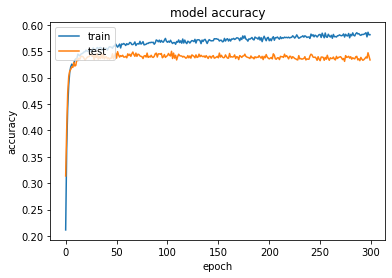
\includegraphics[scale=0.475]{../images/vins_blancs/small_class_accuracy_white.png}
		\caption[Précision du réseau avec toutes les caractéristiques.]
		{\textbf{Précision du réseau avec toutes les caractéristiques}.}
		\label{fig:small-class-accuracy-white}
	\end{minipage}\hfill
	\begin{minipage}[t]{0.48\textwidth}
		\centering
		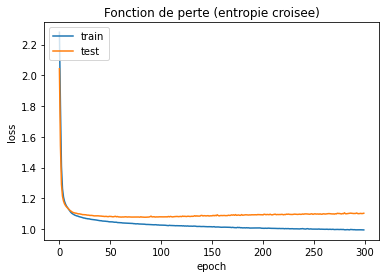
\includegraphics[scale=0.475]{../images/vins_blancs/small_class_loss_white.png}
		\caption[Fonction de perte du réseau avec toutes les caractéristiques.]
		{\textbf{Fonction de perte du réseau avec toutes les caractéristiques}.}
		\label{fig:small-class-loss-white}
	\end{minipage}
\end{figure}

\subsection*{Régression}
\label{sec:regression}

En utilisant l'ensemble des caractéristiques, nous obtenons Erreur Absolue Moyenne (EAM) de 0.5 en apprentissage et en validation.
Nous obtenons les mêmes résultats en utilisant moins de caractéristiques. Ces résultats indiquent clairement qu'il y a une erreur dans le modèle.

\begin{figure}[ht]
	\centering
	\begin{minipage}[t]{0.48\textwidth}
		\centering
		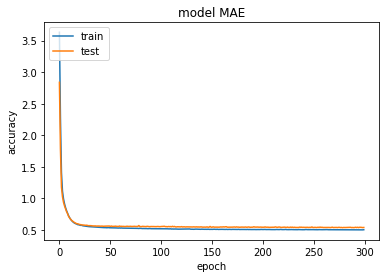
\includegraphics[scale=0.50]{../images/vins_blancs/full_reg_mae_white.png}
		\caption[MAE du réseau]{\textbf{MAE du réseau avec toutes les caractéristiques}.}
		\label{fig:full-reg-mae-white}
	\end{minipage}\hfill
	\begin{minipage}[t]{0.48\textwidth}
		\centering
		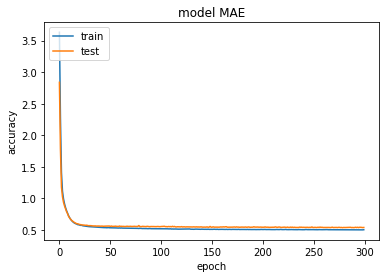
\includegraphics[scale=0.50]{../images/vins_blancs/full_reg_mae_white.png}
		\caption[MAE du réseau]{\textbf{MAE du réseau avec un nombre de caractéristiques limité}.}
		\label{fig:small-reg-mae-white}
	\end{minipage}
\end{figure}